\documentclass{tstextbook}

\begin{document}

\tsbook{Game of Physics游戏策划}
       {Game of Physics小组}
       {Cover Designer}
       {2017}
       {xxxxx}{xxx--xx--xxxx--xx--x}{0.0}
%       {Publisher}
       {余方$\ $周诗蕙$\ $张元一$\ $张冰煜}

%---------------------------------------------------------------------------
% Chapters
%---------------------------------------------------------------------------

%---------------------------------------------------------------------------
\chapter{游戏概述}

\begin{summary}
  Game of Physics (游戏名暂定为《物$|$理》)是一个以开放世界、解谜、RPG和沙盒为主要元素,以物理学为背景,美术风格极简,主要面向14-30岁青年玩家的开放世界解谜类3d游戏。
\end{summary}

\section{游戏运行环境}

游戏主体为exe格式(也可同样的源项目在unity中build成适配于mac系统的dmg格式),运行于PC端,Windows或MacOS环境中。在今后成功做出PC端游戏之后,我们也可能考虑推出手游版本。但是在目前,我们先出PC端。

游戏构架在Unity引擎上,以$C\#$为主要语言编写。

\section{游戏故事情节}

游戏分为实验和理论两个模块。在实验模块,游戏将带领玩家领略真实而丰富的物理世界。以经典力学部分为例,随着游戏的进展,玩家将解锁小球、滑块、不同刚体、陀螺等多个角色,获得绳、链、滑轮等多种道具,可将多个角色组合在地图中,形成多角色RPG扮演,在开放世界地图中探索物理规律之神奇。在这一部分,我们的地图将分为经典地图和沙盒自建地图两块。经典地图将还原物理学史上的种种精彩和经典的实验、思想实验,它是解谜和探索的主线,将撑起游戏的整个主体故事。同时玩家还可以在设定好的地图之外自建地图,玩出超高自由度的沙盒玩法。

物理学是一位用理论和实验两条腿走路的巨人。随着实验的进展,玩家将需要探索物理学理论,以进一步解锁物理世界的大地图。玩家将在探索中获取一步步解锁物理理论的必要工具:数学知识,并籍此习得新技能。技能将可以在理论推理中直接使用,因而当你发现推不下去了的时候,就有可能是缺少技能哦!

随着玩家探索和解谜、推理的进行,玩家将不断解锁原先未知的物理世界。在游戏界面右下角的“物理学地图”中,玩家将拨开云雾,逐渐解锁、点亮物理世界的大地图。在“物理学地图”中,玩家可以通过点击地图中的区域,直接传送到已解锁地图中的某一区域中。



\section{游戏特征}

\subsection{游戏目标}

游戏目标在于探索完物理学大地图。在实验模块中,玩家为了得到预期的实验结果和解锁新实验而自发地思考、规划、克服困难。玩家还会在实验模块的沙盒地图中尽情发挥创造力,创造新奇、有趣、丰富多彩的物理系统。在理论模块中,玩家为了解锁新的物理理论,一步步开拓未知、探索真理而主动地推理公式,并且为了学习新技能而学习必要的数学知识。

\subsection{游戏规则}

游戏中的解谜有一套详尽的逻辑关系网。在精致的安排下,玩家在实验模块下完成某一实验、达到某个预期的实验结果后,将会解锁下一个实验,或者理论模块的icons——灵感小灯泡亮起,提醒玩家有某一物理定律可以解锁。

完成某一实验的条件是达到预期实验结果。为此,我们将对所有实验地图设定成功条件,满足成功条件视为实验成功。

解锁某一理论的条件是推理出这项理论(物理学定律、定理、公式等)。由于推理步骤是按照“技能”来的,即,使用某项数学技能后,会推理至相应的结果,故而数学过程不会存在问题。这样,只要最终结果正确(符合预期),即视为推理成功、理论解锁。

解锁新技能的条件穿插在整个游戏里,依游戏剧情所恰当安排。比如觉得玩到哪里,接下来可以学习微积分了,就在这里将“微积分”技能从“不可见”解锁为“可学习”状态;玩到哪里,接下来必须要微积分的知识了,就在这里要求玩家必须解锁“微积分”技能才能继续。学习数学技能的过程可以设置为一个子关卡、子地图,也可以通过穿插在游戏中的CG展现。

\subsection{反馈系统}

游戏将通过以下反馈系统调动玩家的积极性:

\begin{enumerate}
\item{技能树}

技能是必要的数学知识。如微积分、线性代数、傅里叶变换等等。当游戏进行到解锁相关内容,玩家习得这项技能后,这项技能将在技能树中被点亮,并可直接在接下来的游戏中使用。技能树和技能点将增进玩家的成就感。

\item{物理学大地图}

物理学大地图是一张包含物理学所有内容的地图,类似下图\ref{Fig.map}。但我们会手工重新绘制。玩家每解锁一部分主线内容,将在物理学大地图中显示出来。如图\ref{mapUnlock}。(当然肯定要比这张图精致)

\begin{figure}[H]
\centering 
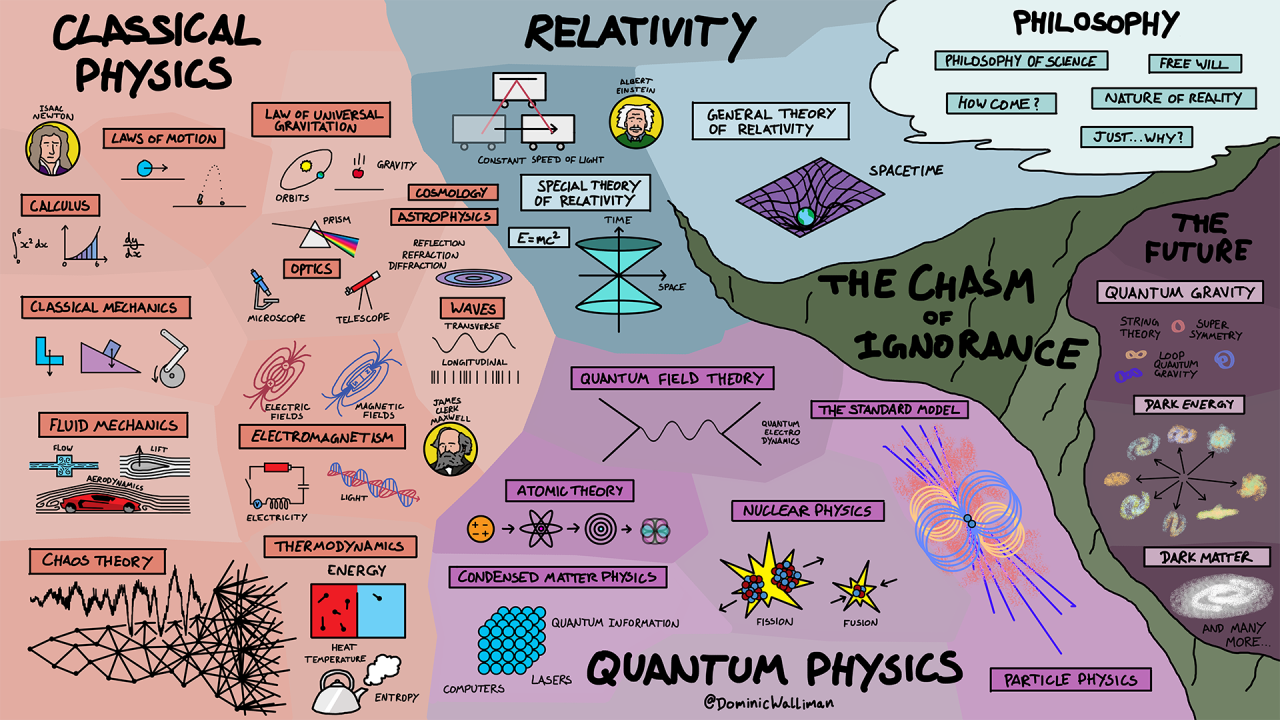
\includegraphics[width=1\textwidth]{MapofPhysics} 
\caption{Map of Physics} 
\label{Fig.map} 
\end{figure}

\begin{figure}[H]
\centering
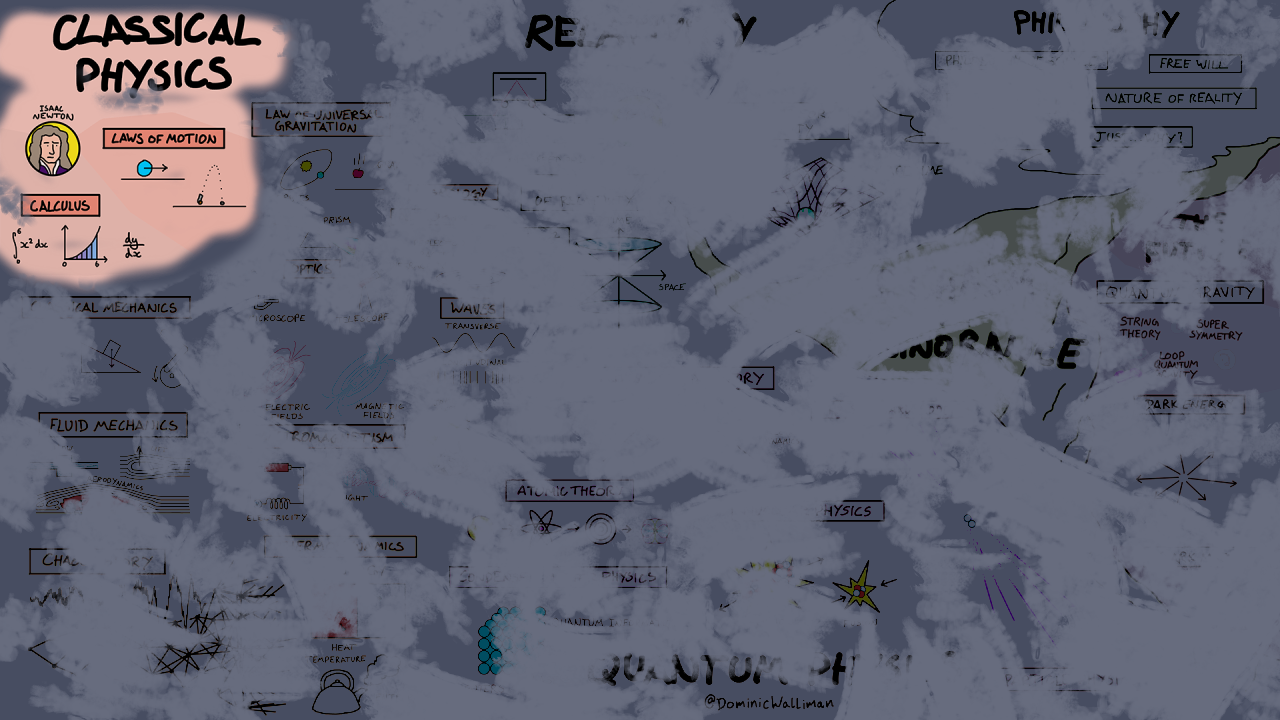
\includegraphics[width=1\textwidth]{UnlockMap} 
\caption{Unlocked Map}
\label{mapUnlock} 
\end{figure}

\item{角色、道具、物品收集}

游戏中,玩家将随着故事的进展逐步解锁不同的角色,如经典力学部分有小球、滑块、杠杆、各种刚体、陀螺等等。这些角色将被玩家永久收入囊中,并且在当前场景里最多可以携带5个角色,以在场景中放置、运动,形成多角色RPG游戏模式。游戏界面的左下角将显示当前场景下的角色信息和状态。

玩家还会随着游戏的进展获得各种道具。这些道具中有用于搭建和组合实验系统的,如绳、链、滑轮等等;也有测量道具和实验仪器,如测速仪、测力计等等。这些道具将被玩家永久收入囊中。在当前场景下,玩家可以随身携带一些道具在界面下方的道具槽中,以随时取用。(类似minecraft中玩家放置一部分道具在场景下方的道具槽中,玩的时候点一下就在当前场景下使用该道具。)

游戏中还会掉落一些物品。这些物品其中一些是彩蛋。见后文。其他类型的物品暂时还没想好。


\item{理论与成就}

已解锁的理论是玩家通过自己的努力解锁的,他们不是教科书上白纸黑字的死的知识,而是玩家自己的发现、自己的推理所获、自己的成就。这将增进玩家的成就感、主动参与感与获得感。

我们可以把重要的理论milestone制作的精美,像宝藏或者勋章,以增强玩家的成就感与获得感。

\item{沙盒与个性化的地图生成}

在实验模块的整个地图中,除了主线故事必有的设计好的地图外,玩家可以使用自己背包里的道具,在周围空白地图中建造自己的实验装置、实验系统,体验沙盒模式的乐趣。建造好的实验装置将保留在玩家的地图中,成为玩家的个性化定制。玩家可以鸟瞰自己目前的地图,尽收眼底的是满满的成就感!

\item{彩蛋$\&$物理背后的故事}

我们会在游戏中穿插一些彩蛋,讲述游戏背后的物理学史上的故事,或致敬物理学上的经典梗(如薛定谔的猫、麦克斯韦妖等等)。彩蛋会并入收集系统,并且提交给steam。玩家之间可以比一比谁收集到的彩蛋多!

\end{enumerate}


\subsection{主动参与}

开放世界的游戏机制将吸引玩家主动参与到探索未知的物理世界中去。

理论模块的解谜和推理的游戏机制将吸引玩家主动探索物理学规律。

游戏的反馈系统将增进玩家的成就感,吸引玩家主动玩下去。

RPG和沙盒模式进一步增加游戏的趣味。

\section{游戏定位}

虽然《物$|$理》以真实的物理科学为背景,希望玩家通过游戏探索和学习物理知识,但是绝不能认为“《物$|$理》是一款教育游戏”而忽视了游戏属性。相反,游戏性必须是《物$|$理》要考虑的重要因素。《物$|$理》是一款游戏,那么它就必须在游戏市场中竞争,它就必须是一款能吸引玩家积极主动投入其中的好游戏。正如某位知乎上的游戏类答主曾说过:“愿世上再没有‘严肃游戏’。”一个好的游戏,不应该通过游戏以外的东西来卖座,来掩饰自己在游戏性上的短板。

游戏的玩家市场定位于14-30岁的年轻人。由于玩家基础的不同,游戏将设置“简单”、“普通”、“困难”和“地狱”四种模式。更难的游戏难度体现在主线要求完成的内容更多、更复杂的实验设计,以及在理论和实验两个模块下均更少的引导和提示上。

我们预计玩家将花5-10小时通关经典力学部分的主线内容。玩家可投入更多时间于更复杂的支线内容、以及沙盒建造中。

\section{游戏风格}

游戏主打极简风格。在极简而审美在线的美术设计中,玩家将免去杂乱元素的干扰,沉浸于物理之美中。同时,极简的风格,搭配上合适、有氛围感的背景音乐,将潜移默化中引导玩家的专注力,使得玩家在行云流水的解谜安排中有沉浸、专注、充满氛围感而丝滑的游戏体验。(技能树icon的设计我还没想好)

\begin{figure}[H]
\centering
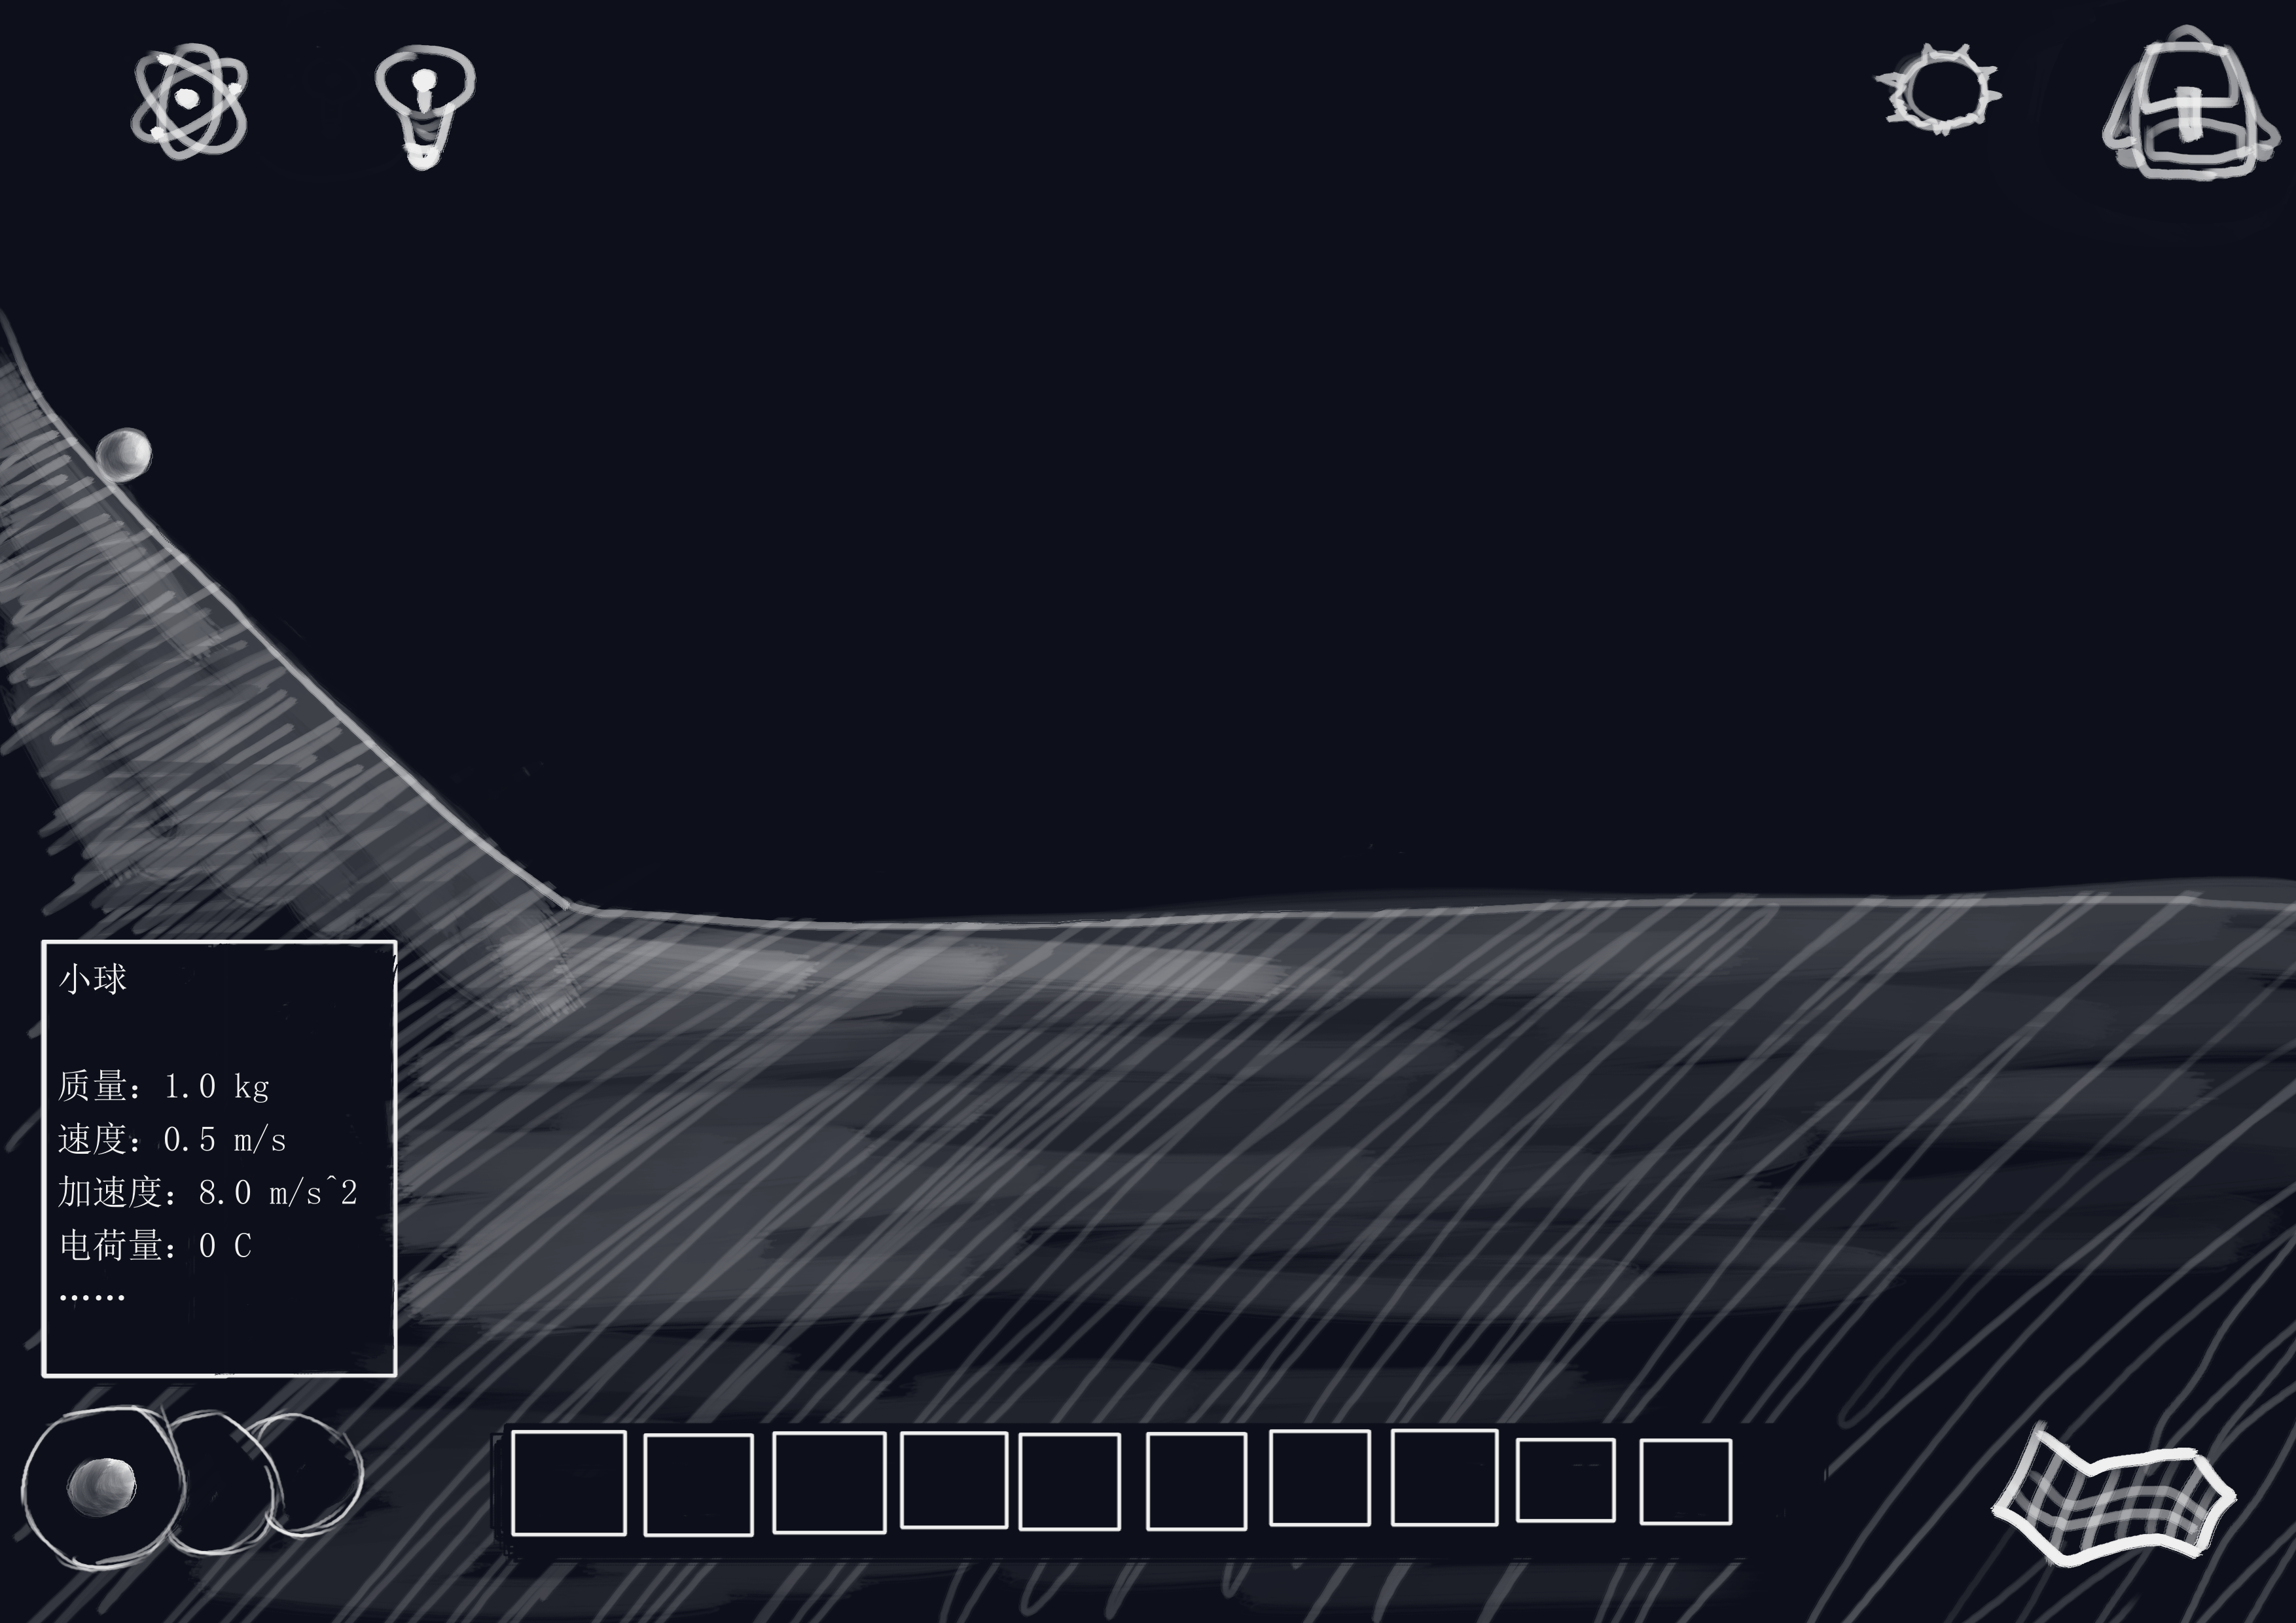
\includegraphics[width=1\textwidth]{MainScene1} 
\caption{游戏界面概念图}
\label{MainScene}
\end{figure}

\begin{figure}[H]
\centering
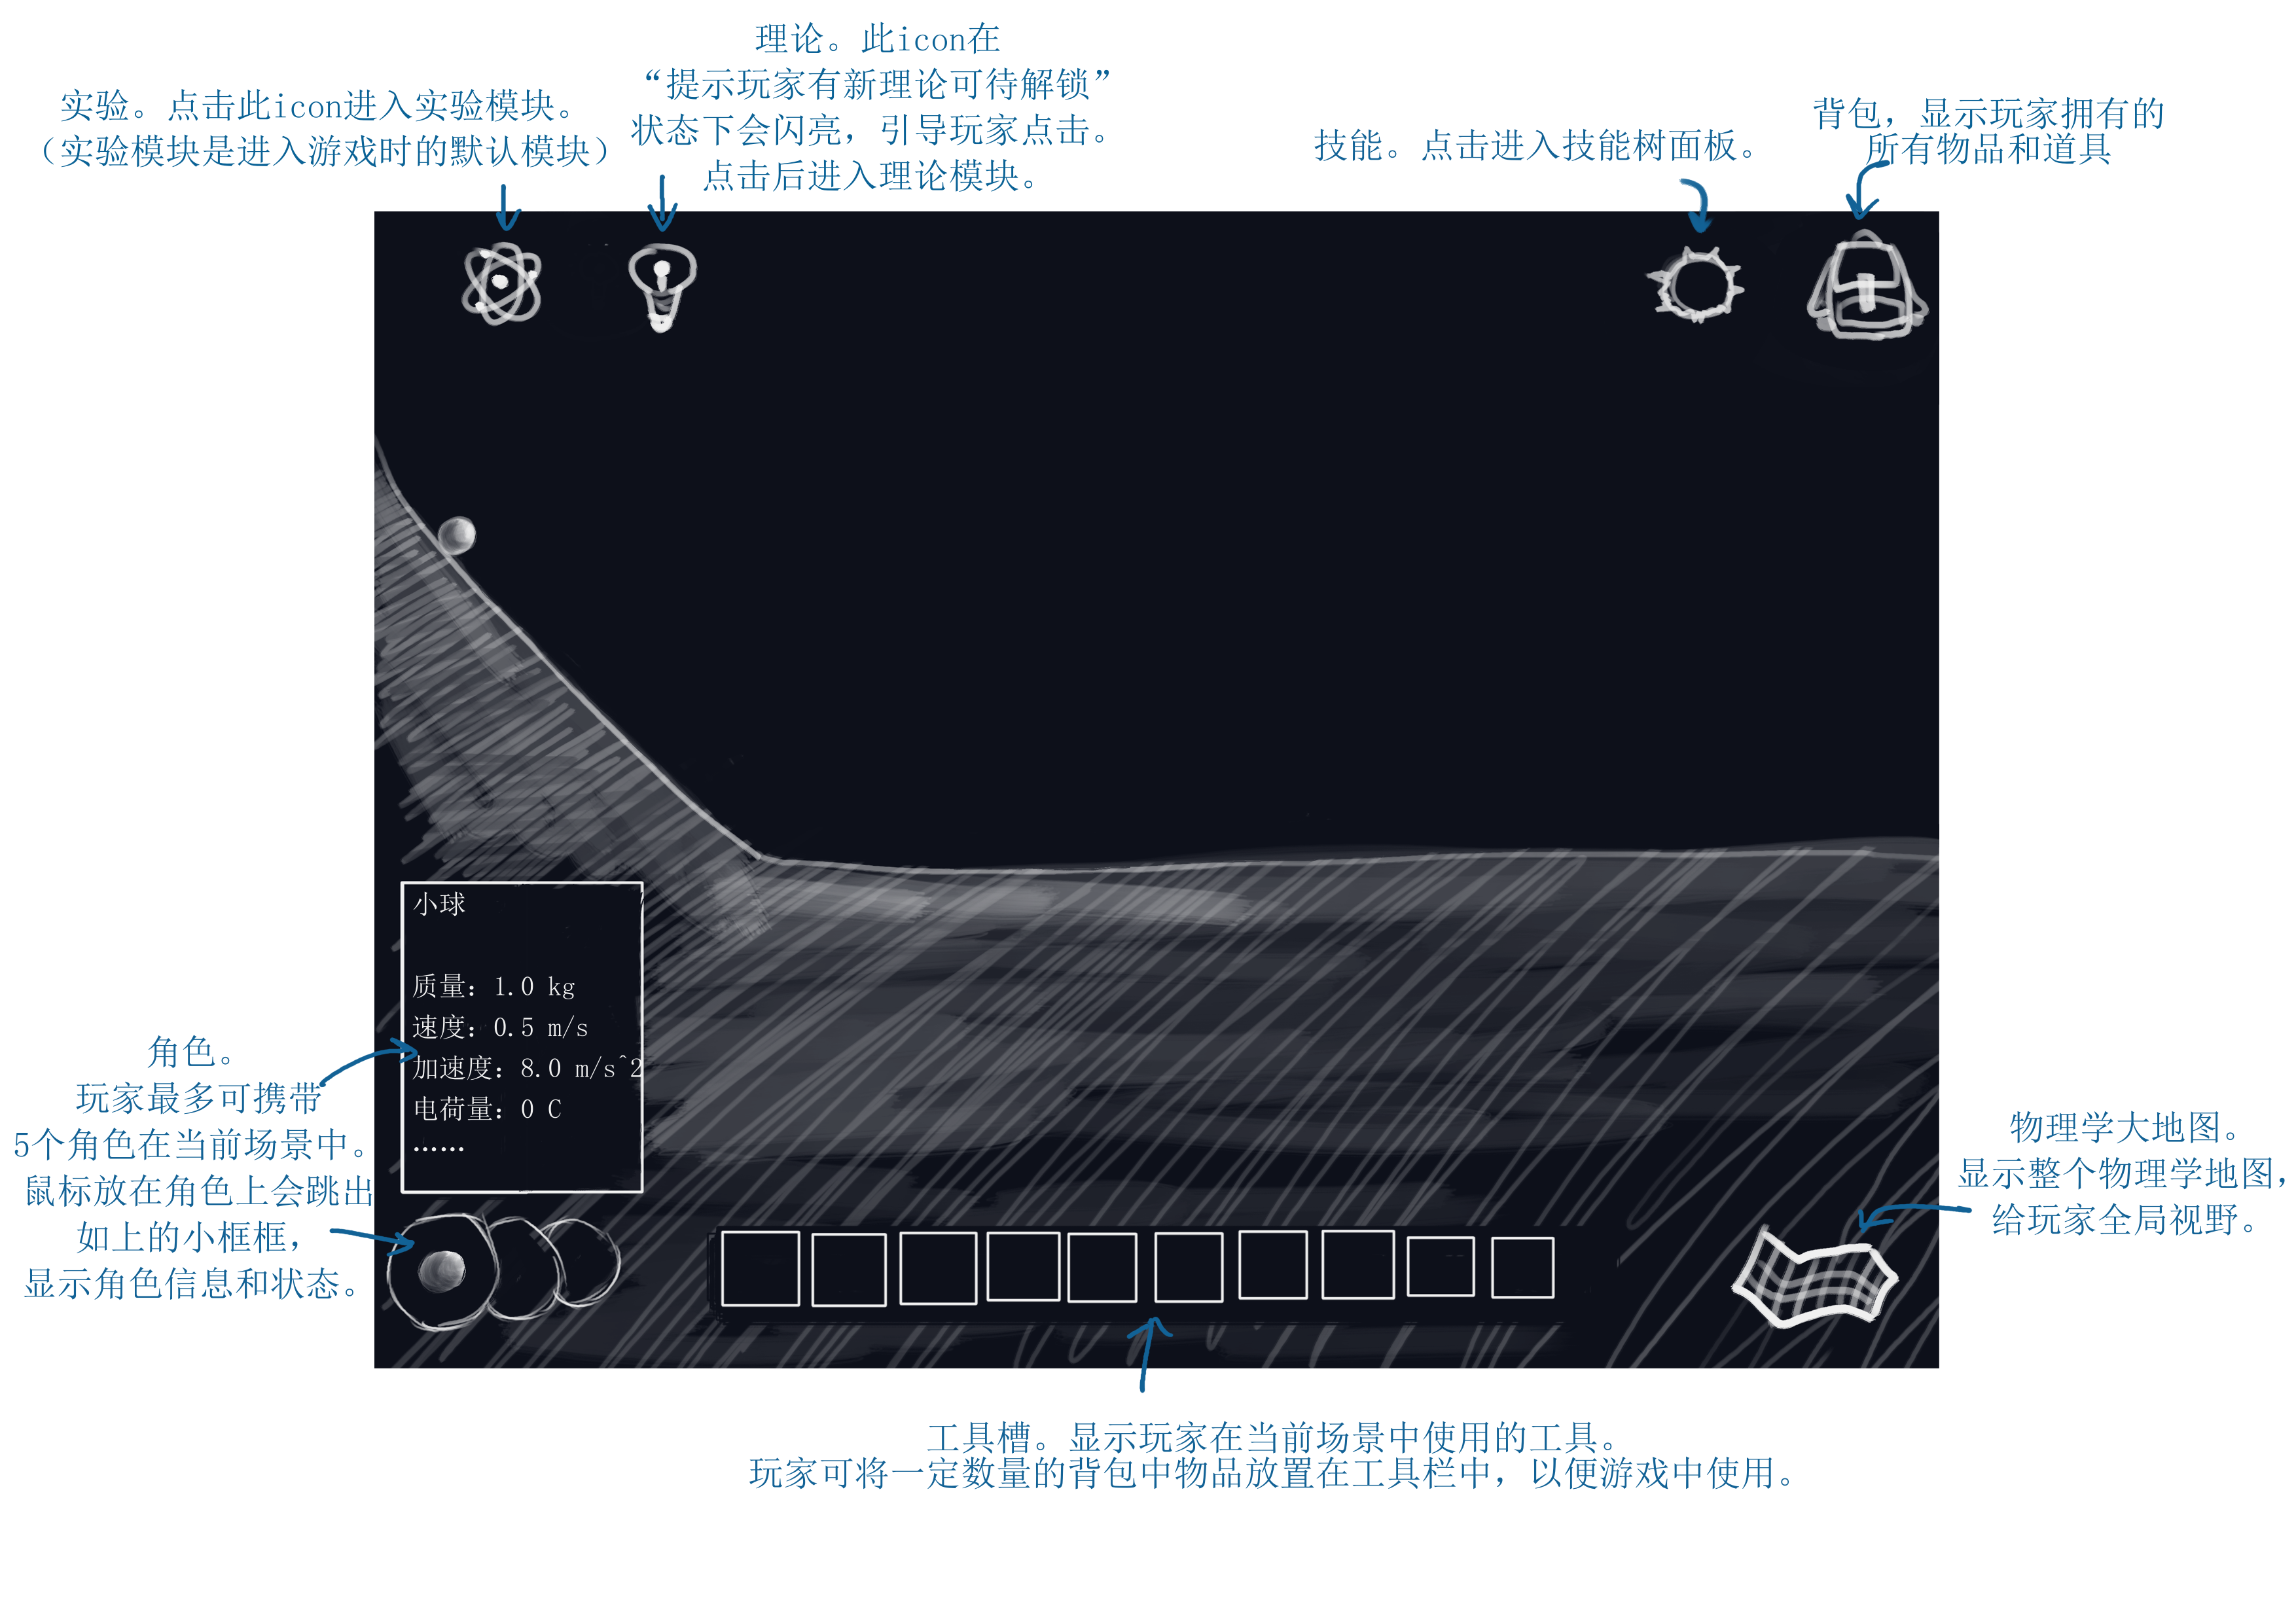
\includegraphics[width=1\textwidth]{MainSceneAnnotated} 
\caption{概念图说明}
\label{MainScene}
\end{figure}

《物$|$理》的音乐风格可以设计成古典+现代电子/重金属音乐的融合.

%---------------------------------------------------------------------------
\chapter{游戏机制}

\begin{summary}
《物$|$理》融合了开放世界、解谜、RPG和沙盒机制。
\end{summary}

\section{游戏性设计}

\begin{enumerate}

\item{关注点}



\end{enumerate}


\section{游戏操作}

\subsection{角色控制:在开放的物理学世界中做实验}

玩家可以用鼠标和键盘控制角色,在开放的物理学世界中自由探索、实验,发现奇妙的物理现象。

\begin{enumerate}

\item{切换当前角色}

当前场景下的所有角色将显示在左下角,玩家可以点击要选中的角色的标志,切换当前移动和施力等操作的默认对象。玩家也可以通过键盘上的1、2、3、4来完成快捷操作。

\item{拎起、移动、释放角色}

玩家用鼠标左键点击角色时,将拎起角色,而后角色将随鼠标在场景中移动。当玩家再次点击鼠标左键时,角色在该位置由静止释放。玩家也可以通过键盘的shift + W/A/S/D或者$\leftarrow\uparrow\downarrow\rightarrow$实现此操作。

\item{给角色施加作用力}

玩家用鼠标右键按住角色并拖拽,将在拖拽方向对角色施加一个作用力。玩家滑动鼠标中键滚轮,将改变力的大小。玩家也可以用键盘的W/A/S/D或者$\uparrow\leftarrow\downarrow\rightarrow$实现该操作。

\item{临时角色}

在有些地图上,玩家会解锁临时角色。比如《镜中人》实验中,玩家将解锁临时角色:一位小矿工。临时角色可能有不同于一般角色的特殊操作,将在后文中特殊说明。

\end{enumerate}

\subsection{查看角色属性和信息}

玩家将鼠标放置在左下角的角色icon上时,将以icon上方出现小方框的形式显示角色属性和相关信息。

\subsection{放置和搭建实验地图}

在有些地图中,实验装置未搭建完全。玩家需要利用自己背包里已有的道具,辅助搭建实验地图。

\begin{enumerate}

\item{将道具从背包放入道具栏中}

玩家点击游戏界面右上角的“背包”icon,将打开背包。玩家点击背包的格子中自己要选择的道具,再点击游戏界面下方的道具栏空格,将把道具从背包放入道具栏中。若玩家点击了道具栏中一个已装有其他道具的非空格子,将实现替换操作。玩家也可以反过来先点击道具栏中的道具,再点击背包中的空格,将道具栏中的道具放回背包内。玩家也可以通过双击实现相同操作。

\item{在地图中使用道具}

玩家点击道具栏中要选择的道具,将拎起道具,道具将随鼠标在地图上移动,直到玩家在地图某位置上再次点击鼠标时,将在该位置放置道具。在一些地图上的特殊位置,如能将道具和角色连接(比如用轻绳连接小球)的位置上,玩家将鼠标靠近时会自动吸附,并在接触位置高亮显示以作强调。玩家就能知道这些是特殊位置。

\end{enumerate}

\subsection{暂停物理过程}

玩家可按下键盘上的空格键暂停物理过程,以检查自己的实验装置,或者仔细研究当前场面。在暂停模式下玩家仍能移动物体,但物体将不再物理运动。再次按下空格键后一切继续运动。

游戏不建议玩家在实验进行到一半时移动角色或道具,因此会在引导中提醒玩家避免此类操作。(或者也可以只允许在场景中的特定区域内移动角色或道具,以避免玩家在实验中途打乱实验装置。)

\subsection{用测量道具测量}

测量道具(如尺子、测速仪、测力计等)和其他道具一样放置在背包里(可以分开放置,如背包中分成“测量”、“道具”两个夹层),玩家可以自由选择要使用的测量道具放入道具栏中。当把测量道具移动到要测量的对象(如某角色)上时,将显示测量结果,并绘制结果随时间变化的曲线。

如:要测量小球速度,则将测速仪放在小球上。然后在游戏界面的左上方将显示测速仪icon,并且开始绘制小球的速度曲线。

\subsection{学习和使用技能,完成理论推理}

\begin{enumerate}

\item{学习技能,点亮技能树}

在特定时机下,技能树中的某个格子将被解锁,提醒玩家此技能可以学习。

玩家点击该格子,将进入技能学习CG或临时关卡中。

\item{在推理中使用技能}

\end{enumerate}

\subsection{跑地图}

玩家将鼠标放置于屏幕上下左右边缘时,将在此方向上移动地图。鼠标中键滚轮可控制视角大小。

视角移动操作仅限于已解锁的地图之内。

\section{用户界面}



\section{玩家交互}


%---------------------------------------------------------------------------
\chapter{游戏元素}

\begin{summary}
《物$|$理》中有角色、道具和技能元素。
\end{summary}

\section{角色}

\begin{enumerate}

\item{小球}

\item{滑块}

\item{杆}

\item{陀螺}

\item{圆盘}

\end{enumerate}

\section{道具}

\subsection{普通道具}

\begin{enumerate}

\item{轻绳}

\item{滑轮}

\item{轻杆}

\item{链}

\item{钮连}

\end{enumerate}

\subsection{测量道具}

\begin{enumerate}

\item{尺子}

\item{测速仪}

\item{测力计}

\end{enumerate}

\section{技能}

\begin{enumerate}

\item{微分}

\item{积分}

\item{傅里叶变换}

\end{enumerate}

\section{场景}

\begin{enumerate}

\item{比萨斜塔}

\item{微摩擦抛物面坑}

\end{enumerate}

%---------------------------------------------------------------------------
\chapter{游戏的故事背景}

\begin{summary}

\end{summary}

%---------------------------------------------------------------------------
\chapter{游戏过程}

\begin{summary}

\end{summary}

\section{经典力学demo}

\subsection{第一幕}

开场。三个小球从比萨斜塔上由静止释放,同时落地,然后滚上不同斜坡。

\begin{figure}[H]
\centering 
\includegraphics[width=1\textwidth]{Chapter1_1} 
\caption{第一幕} 
\label{1.1} 
\end{figure}

这时候产生了几个问题:

\begin{enumerate}
\item{三个小球为什么同时落地?}
\item{绿球和蓝球为什么滚上了同样的高度?(释放时的高度?)}
\item{黑球为什么会保持运动状态一直滚下去?}
\end{enumerate}

问题收录至日志中。为了解答这些问题,接下来由玩家你自由探索。

\subsection{牛顿定律}

\begin{enumerate}

\item{黑球惯性实验}

现在有三个相同的黑球,在三层平面上。对它们施加同样的拉力,到起始位置时撤去。三个平面摩擦系数不同。三个小球运动了不同的距离。实验结束后,解锁“惯性定律”。同时问题1.3得解。

\item{F=ma实验}

做3-5组实验,测量合力F,质量m和加速度a(加速度通过对速度曲线求导得到),完成后画出F-m*a图,得到F=ma。

\item{作用力和反作用力}

做3-5组实验,对两个相互作用的物体分别受力分析,完成后得到牛顿第三定律:作用力和反作用力相等。

\end{enumerate}

\subsection{参考系、惯性参考系与伽利略变换}

\begin{enumerate}

\item{台球实验}

致敬刘慈欣《三体》1中的《台球》,和阿西莫夫的短篇小说《台球》。完成后得到“物理学定律在一切惯性系中等效”。

\end{enumerate}

\subsection{非惯性系}

\begin{enumerate}

\item{傅科摆}

证明地球自转及由于地球自转引起的科里奥利力(地转偏向力)。玩家将以此为契机探索非惯性系下的科里奥利力公式。

傅科摆实验还可以验证能量守恒(如未验证)、以及解锁波动力学部分(如未解锁),和经典天体物理部分(如未解锁)。

\begin{figure}[H]
\centering 
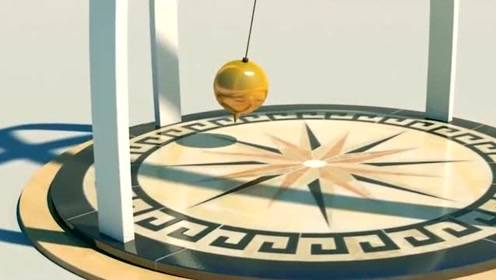
\includegraphics[width=1\textwidth]{Foucault} 
\caption{Foucault's Pendulum} 
\label{Foucault} 
\end{figure}

傅科摆还可以用分析力学探究。(假如玩家解锁了分析力学的话。)

\item{陀螺的进动}

玩家获得新角色:陀螺。让陀螺在地图上旋转,玩家将发现陀螺进动的现象。玩家将籍此探索进动的规律。该支线地图需要先解锁刚体力学而后解锁。

\begin{figure}[H]
\centering 
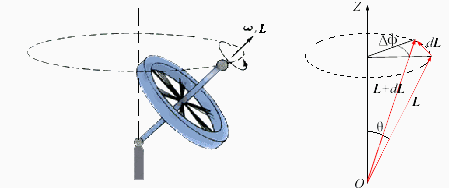
\includegraphics[width=1\textwidth]{processing} 
\caption{陀螺的进动} 
\label{processing} 
\end{figure}

陀螺的进动还可以用分析力学探究。(假如玩家解锁了分析力学的话。)

\end{enumerate}

\subsection{能量、功能关系、动能定理、机械能守恒}

\begin{enumerate}

\item{镜中人实验}

致敬杰弗里·A·兰迪斯 《镜中人》。一个微摩擦的抛物面大坑。一个矿工被困在了坑里,想办法出去。

玩家获得临时角色:一个小人。可以奔跑、跳跃、蹲下、翻滚、旋转(在满足物理规律的前提下)。所有这些动作会消耗体力。玩家需要在小人的体力耗尽前逃出矿坑,否则实验失败,被锁定。直到玩家接下来获得更多经验、成长了以后才能再次解锁。

\begin{figure}[H]
\centering 
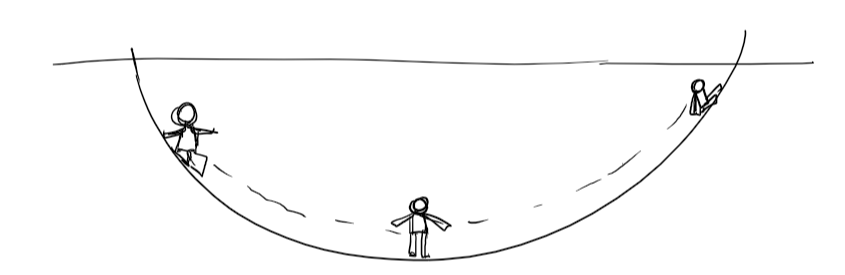
\includegraphics[width=1\textwidth]{mirror} 
\caption{镜中人} 
\label{mirror} 
\end{figure}

\subsection{动量定理、动量守恒}

\subsection{力矩和角动量}

\subsection{质心、质心系、刚体力学}

\subsection{经典天体物理}



\end{enumerate}

%---------------------------------------------------------------------------
% Bibliography
%---------------------------------------------------------------------------

\addcontentsline{toc}{chapter}{\textcolor{tssteelblue}{Literature}}
\printbibliography{}

%---------------------------------------------------------------------------
% Index
%---------------------------------------------------------------------------

\printindex

\end{document}
